\section{Mean field: the superfluid state and its spinor solutions}
\label{sec:meanfield}

\subsection{The mean-field approximation}

Two exact identities split each quartic term into a part linear in a bilinear and the square of
its fluctuation:
\begin{equation}
\begin{aligned}
G^S_{U2}(\bar\Psi_{U2}\Psi_{U2})^2={}&2G^S_{U2}\langle\bar\Psi_{U2}\Psi_{U2}\rangle\,\bar\Psi_{U2}\Psi_{U2}\\
&-G^S_{U2}\langle\bar\Psi_{U2}\Psi_{U2}\rangle^2\\
&+G^S_{U2}\big(\bar\Psi_{U2}\Psi_{U2}-\langle\bar\Psi_{U2}\Psi_{U2}\rangle\big)^2,\\
G^P_{U2}\Phi^{+\dagger}_{U2}\Phi^+_{U2}={}&G^P_{U2}\langle\Phi^+_{U2}\rangle^*\Phi^+_{U2}
+G^P_{U2}\Phi^{+\dagger}_{U2}\langle\Phi^+_{U2}\rangle\\
&-G^P_{U2}|\langle\Phi^+_{U2}\rangle|^2\\
&+G^P_{U2}\big(\Phi^+_{U2}-\langle\Phi^+_{U2}\rangle\big)^\dagger\\
&\quad\times\big(\Phi^+_{U2}-\langle\Phi^+_{U2}\rangle\big),
\end{aligned}
\label{eq:split}
\end{equation}
where $\langle\ \rangle$ is the expectation value in the ground state. The mean-field
approximation drops the squares of the fluctuations (the last term of each line). With the
\emph{effective mass} and the \emph{pair field}
\begin{equation}
M_{U2}=m_{U2}-2G^S_{U2}\langle\bar\Psi_{U2}\Psi_{U2}\rangle,\qquad
\Delta_{U2}=G^P_{U2}\langle\Phi^+_{U2}\rangle,
\label{eq:MD}
\end{equation}
and the gauge fields at their mean values, zero (the condensate is an $SU(2)_{U2}$ singlet, and
the $U(1)_{U2}$ charge is neutralized, Sec.~\ref{sec:lagrangian}), the Lagrangian becomes
\begin{equation}
\begin{aligned}
\mathcal L^{\rm MF}_{U2}={}&\bar\Psi_{U2}\big(i\gamma^A_{1671}\partial_A-M_{U2}\big)\Psi_{U2}
+\Delta^*_{U2}\Phi^+_{U2}+\Delta_{U2}\Phi^{+\dagger}_{U2}\\
&-\frac{|\Delta_{U2}|^2}{G^P_{U2}}-\frac{(M_{U2}-m_{U2})^2}{4G^S_{U2}},
\end{aligned}
\label{eq:LMF}
\end{equation}
(the constants follow from $\langle\bar\Psi_{U2}\Psi_{U2}\rangle=(m_{U2}-M_{U2})/(2G^S_{U2})$ and
$\langle\Phi^+_{U2}\rangle=\Delta_{U2}/G^P_{U2}$), and Eq.~\eqref{eq:EL} becomes the mean-field
Dirac equation
\begin{equation}
i\gamma^A_{1671}\partial_A\Psi_{U2}=M_{U2}\Psi_{U2}+\Delta_{U2}\tilde\Psi_{U2}.
\label{eq:MFDirac}
\end{equation}
The same equations are the saddle point of the path integral after a Hubbard--Stratonovich
transformation~\cite{Hubbard1959,Stratonovich1957}, which introduces $M_{U2}$ and $\Delta_{U2}$ as
auxiliary fields; the mean-field approximation is the leading order of that formulation, as in
the theories of Bardeen, Cooper and Schrieffer~\cite{BCS1957} and of Nambu and
Jona-Lasinio~\cite{NJL1961}. The fluctuations of the auxiliary fields about the saddle point are
the collective modes of Sec.~\ref{sec:breaking}.

\subsection{The Bogoliubov--de Gennes matrix}

In a large periodic box of volume $\mathrm{Vol}_{U2}$ the Fourier components of the fields at a
fixed time are $\psi^1_{U2}(\vec q)=\mathrm{Vol}_{U2}^{-1/2}\int d^7x\,\exp(-i\vec q\cdot\vec x)\,
\psi^1_{U2}$, and the same for $\psi^2_{U2}$. The Hamiltonian of Eq.~\eqref{eq:LMF}, minus
$\mu_{U2}N_{U2}$, couples $\psi^1_{U2}$ at the momentum $\vec q$ only with $\psi^2_{U2}$ at
$-\vec q$. With the 32-component \emph{Nambu spinor}
$\mathcal N_{U2}(\vec q)=\big(\psi^1_{U2}(\vec q),\ \psi^2_{U2}(-\vec q)^{\dagger T}\big)$, whose lower
half holds the Hermitian conjugates of the components of $\psi^2_{U2}(-\vec q)$,
\begin{equation}
\begin{aligned}
H^{\rm MF}_{U2}-\mu_{U2}N_{U2}={}&\sum_{\vec q}\mathcal N^\dagger_{U2}\mathsf H_{U2}\mathcal N_{U2}\\
&+\mathrm{Vol}_{U2}\Big[\frac{|\Delta_{U2}|^2}{G^P_{U2}}+\frac{(M_{U2}-m_{U2})^2}{4G^S_{U2}}\Big],
\end{aligned}
\label{eq:HMF}
\end{equation}
with the sum over the momenta of the box and the $32\times32$ Bogoliubov--de Gennes matrix
\begin{equation}
\begin{aligned}
\mathsf H_{U2}(\vec q)&=\begin{pmatrix}\mathsf h_{U2}-\mu_{U2} & \Delta_{U2}C^+_{1671}\\
\Delta^*_{U2}C^+_{1671} & \mu_{U2}-\beta_{1671}\mathsf h_{U2}\beta_{1671}\end{pmatrix},\\
\mathsf h_{U2}&=\alpha^j_{1671}q^j+\beta_{1671}M_{U2},
\end{aligned}
\label{eq:BdG}
\end{equation}
where $\mu_{U2}$ in a block stands for $\mu_{U2}\mathsf 1_{16}$, and
$-\beta_{1671}\mathsf h_{U2}\beta_{1671}=\alpha^j_{1671}q^j-\beta_{1671}M_{U2}$. The upper left block is the
Dirac Hamiltonian of $\psi^1_{U2}$ in momentum space, minus the chemical potential. The lower right
block comes from the same terms for $\psi^2_{U2}(-\vec q)$:
written with the Hermitian-conjugate components, the bilinear of $\psi^2_{U2}$ with a
$16\times16$ matrix turns into minus the bilinear of the transposed matrix (one anticommutation
per term), and $(\mathsf h_{U2}(-\vec q)-\mu_{U2}\mathsf 1_{16})^T=-\alpha^j_{1671}q^j+\beta_{1671}M_{U2}-\mu_{U2}\mathsf 1_{16}$
because $\alpha^j_{1671}$ and $\beta_{1671}$ are symmetric; the constant that the anticommutation
produces cancels in the charge-symmetric order, and $\mathrm{Tr}\,\mathsf H_{U2}=0$. The
off-diagonal blocks come from $\Delta^*_{U2}\Phi^+_{U2}+\Delta_{U2}\Phi^{+\dagger}_{U2}$. The
Heisenberg equation of motion, $i\partial_4\mathcal N_{U2}=\mathsf H_{U2}\mathcal N_{U2}$, is
Eq.~\eqref{eq:MFDirac} in Hamiltonian form (multiply Eq.~\eqref{eq:MFDirac} by
$\beta_{1671}$). The spectrum does not depend on the phase of $\Delta_{U2}$ (R3-U1): the phase is
removed by multiplying $\psi^1_{U2}$ and $\psi^2_{U2}$ by the same constant phase. Below
$\Delta_{U2}$ is real and positive unless said otherwise.

\subsection{Spectrum and spinor solutions}
\label{sec:spectrum}

\emph{Invariant planes.} Let $\mathsf e^\pm_{U2}$ be a real normalized eigenvector of
$\mathsf h_{U2}(\vec q)$ with the eigenvalue $\pm\varepsilon_{U2}$,
$\varepsilon_{U2}=(q^2+M^2_{U2})^{1/2}$; there are eight of each sign, because
$\mathsf h_{U2}^2=\varepsilon_{U2}^2\mathsf 1_{16}$ and $\mathrm{Tr}\,\mathsf h_{U2}=0$. From
$\beta_{1671}\alpha^j_{1671}=-\alpha^j_{1671}\beta_{1671}$ it follows that
$(\alpha^j_{1671}q^j-\beta_{1671}M_{U2})\beta_{1671}\mathsf e^\pm_{U2}=
-\beta_{1671}\mathsf h_{U2}\mathsf e^\pm_{U2}=\mp\varepsilon_{U2}\beta_{1671}\mathsf e^\pm_{U2}$, and
$C^+_{1671}=\beta_{1671}$ maps $\mathsf e^\pm_{U2}$ to $\beta_{1671}\mathsf e^\pm_{U2}$ and back. So the
plane spanned by $(\mathsf e^\pm_{U2},0)$ and $(0,\beta_{1671}\mathsf e^\pm_{U2})$ is invariant, and
on it $\mathsf H_{U2}$ is the $2\times2$ matrix
\begin{equation}
\begin{pmatrix}\xi^\pm_{U2}&\Delta_{U2}\\ \Delta_{U2}&-\xi^\pm_{U2}\end{pmatrix},\qquad
\xi^\pm_{U2}=\pm\varepsilon_{U2}-\mu_{U2},
\label{eq:block}
\end{equation}
with the eigenvalues $\pm[(\xi^\pm_{U2})^2+\Delta_{U2}^2]^{1/2}$. The 16 planes (one for each
eigenvector of $\mathsf h_{U2}$) are mutually orthogonal and fill the 32 dimensions. The
eigenvalues of $\mathsf H_{U2}$ are therefore $\pm E^+_{U2}$ and $\pm E^-_{U2}$, each eightfold,
\begin{equation}
E^\pm_{U2}=\big[(\varepsilon_{U2}\pm\mu_{U2})^2+\Delta_{U2}^2\big]^{1/2}
\label{eq:Epm}
\end{equation}
(R3-C1). The planes of the positive-energy eigenvectors $\mathsf e^+_{U2}$ (particles) carry
$E^-_{U2}$, those of $\mathsf e^-_{U2}$ (antiparticles) carry $E^+_{U2}$. The eigenvectors, the
spinor solutions of the mean-field equations, are explicit (R3-C3):
\begin{equation}
\begin{aligned}
+E^\mp_{U2}:&\quad \big(u^\pm_{U2}\,\mathsf e^\pm_{U2},\ v^\pm_{U2}\,\beta_{1671}\mathsf e^\pm_{U2}\big),\\
-E^\mp_{U2}:&\quad \big(-v^\pm_{U2}\,\mathsf e^\pm_{U2},\ u^\pm_{U2}\,\beta_{1671}\mathsf e^\pm_{U2}\big),
\end{aligned}
\label{eq:spinors}
\end{equation}
with the Bogoliubov coefficients $u^\pm_{U2}=[(1+\xi^\pm_{U2}/E^\mp_{U2})/2]^{1/2}$ and
$v^\pm_{U2}=[(1-\xi^\pm_{U2}/E^\mp_{U2})/2]^{1/2}$, which satisfy
$(u^\pm_{U2})^2+(v^\pm_{U2})^2=1$ and $2u^\pm_{U2}v^\pm_{U2}=\Delta_{U2}/E^\mp_{U2}$. As functions
of space and time, $\mathcal N_{U2}\propto(u^\pm_{U2}\mathsf e^\pm_{U2},v^\pm_{U2}\beta_{1671}\mathsf
e^\pm_{U2})\exp(i\vec q\cdot\vec x-iE^\mp_{U2}x4)$ and its partner of negative energy solve the
self-interacting Dirac equation~\eqref{eq:MFDirac} in Hamiltonian form, for every $\vec q$: these
are the spinor solutions that the task asks for. Each of them mixes a particle of $\psi^1_{U2}$
with a hole of $\psi^2_{U2}$ of opposite momentum, with the weights $u^\pm_{U2}$ and $v^\pm_{U2}$.

\emph{The same spectrum from anticommutators.} Write $\mathsf H_{U2}$ as the sum of four real
symmetric matrices: the kinetic part $\mathrm{diag}(\alpha^j_{1671}q^j,\alpha^j_{1671}q^j)$, the mass
part $M_{U2}\mathsf V^3_{U2}$ with $\mathsf V^3_{U2}=\mathrm{diag}(\beta_{1671},-\beta_{1671})$, the
chemical-potential part $-\mu_{U2}\,\mathrm{diag}(\mathsf 1_{16},-\mathsf 1_{16})$, and the pair part
$\Delta_{U2}\mathsf V^1_{U2}$ with $\mathsf V^1_{U2}=\big(\begin{smallmatrix}0&C^+_{1671}\\
C^+_{1671}&0\end{smallmatrix}\big)$. The kinetic, the mass and the pair part anticommute with each
other (R3-A13); the chemical-potential part commutes with the first two and anticommutes with the
third. Hence all cross terms of the square vanish except those of the chemical-potential part
with the kinetic and the mass part, and
$\mathsf H_{U2}^2=(\varepsilon_{U2}^2+\mu_{U2}^2+\Delta_{U2}^2)\mathsf 1_{32}+2\mathsf Y_{U2}$, where
$\mathsf Y_{U2}=-\mu_{U2}\,\mathrm{diag}(\mathsf 1_{16},-\mathsf 1_{16})\,[\mathrm{diag}(\alpha^j_{1671}q^j,\alpha^j_{1671}q^j)+M_{U2}\mathsf V^3_{U2}]$
has the square $\mu^2_{U2}\varepsilon^2_{U2}\mathsf 1_{32}$. The eigenvalues of $\mathsf H^2_{U2}$ are
$\varepsilon^2_{U2}+\mu^2_{U2}+\Delta^2_{U2}\pm2\mu_{U2}\varepsilon_{U2}=(E^\pm_{U2})^2$.

\emph{The pseudoscalar pair, for comparison.} With $C^-_{1671}$ in place of $C^+_{1671}$ the pair
part \emph{commutes} with the mass part (R3-A13), and the same computation gives $\mathsf
H^2_{U2}=(\varepsilon^2_{U2}+\mu^2_{U2}+\Delta^2_{U2})\mathsf 1_{32}+2\mathsf Y'_{U2}$ with
$(\mathsf Y'_{U2})^2=(\mu^2_{U2}\varepsilon^2_{U2}+M^2_{U2}\Delta^2_{U2})\mathsf 1_{32}$, where $\mathsf
Y'_{U2}$ adds the product of the mass and the pair part to $\mathsf Y_{U2}$; hence the eigenvalues
\begin{equation}
\pm\big[\varepsilon^2_{U2}+\mu^2_{U2}+\Delta^2_{U2}\pm2(\mu^2_{U2}\varepsilon^2_{U2}+M^2_{U2}\Delta^2_{U2})^{1/2}\big]^{1/2}
\label{eq:Cminus}
\end{equation}
(R3-C2). At a Fermi surface the difference matters (R3-C6): for the spin-zero pair the smallest
quasi-particle energy is $\Delta_{U2}$, reached at $\varepsilon_{U2}=\mu_{U2}$; for the
pseudoscalar pair the minimum of Eq.~\eqref{eq:Cminus} is
\begin{equation}
\Delta_{U2}\big(1-M^2_{U2}/\mu^2_{U2}\big)^{1/2}=\Delta_{U2}\,q^F_{U2}/\mu_{U2},
\label{eq:FSgap}
\end{equation}
($q^F_{U2}=(\mu^2_{U2}-M^2_{U2})^{1/2}$ the Fermi momentum), which vanishes in the
non-relativistic limit $q^F_{U2}\ll M_{U2}$. The pseudoscalar pair cannot open a gap at a slow
Fermi surface, in accord with Eq.~\eqref{eq:restframe}; the spin-zero pair opens the full gap.
Figure~\ref{fig:spectrum} shows the three cases.

\begin{figure*}[t]
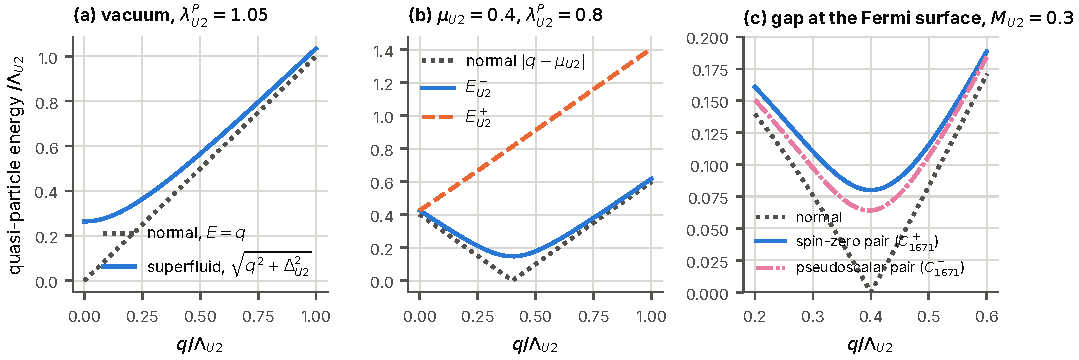
\includegraphics[width=\textwidth]{../figures/fig_r3_spectrum.pdf}
\caption{Quasi-particle energies (units $\Lambda_{U2}=1$, $m_{U2}=0$ in (a) and (b)).
(a)~Vacuum: normal state, energy $q$, and superfluid, $(q^2+\Delta^2_{U2})^{1/2}$, at
$\lambda^P_{U2}=1.05$, where the minimum of the effective potential has
$\Delta_{U2}={{GENM:num_Delta_spectrum_vac}}$. (b)~Finite density, $\mu_{U2}=0.4$, $\lambda^P_{U2}=0.8$
(below the critical coupling of the vacuum): the normal energies $|q-\mu_{U2}|$ and $q+\mu_{U2}$,
and $E^-_{U2}$, $E^+_{U2}$ of Eq.~\eqref{eq:Epm} with the self-consistent
$\Delta_{U2}={{GENM:num_Delta_spectrum_den}}$. (c)~Near a Fermi surface with $M_{U2}=0.3$,
$\mu_{U2}=0.5$, $\Delta_{U2}=0.08$: the spin-zero pair opens the full gap $\Delta_{U2}$, the
pseudoscalar pair only $\Delta_{U2}q^F_{U2}/\mu_{U2}=0.064$ [Eq.~\eqref{eq:FSgap}].}
\label{fig:spectrum}
\end{figure*}

\subsection{The superfluid ground state and the gap equation}

In each invariant plane the occupied state is the eigenvector of negative eigenvalue. For an
eigenvector $\mathsf e^\pm_{U2}$ of $\mathsf h_{U2}(\vec q)$ define the mode annihilators
$a_{U2}=(\mathsf e^\pm_{U2})^T\psi^1_{U2}(\vec q)$ and $d_{U2}=(\beta_{1671}\mathsf
e^\pm_{U2})^T\psi^2_{U2}(-\vec q)$, and the pair creator $b^\dagger_{U2}=a^\dagger_{U2}d^\dagger_{U2}$; in the
plane the Hamiltonian is $(a^\dagger_{U2},d_{U2})$ times the matrix~\eqref{eq:block} times
$(a_{U2},d^\dagger_{U2})^T$. The ground state is
\begin{equation}
|\mathrm{SF}_{U2}\rangle=\prod_{\vec q}\ \prod_{\mathsf e^\pm_{U2}}\big(u^\pm_{U2}-v^\pm_{U2}\,b^\dagger_{U2}\big)\,|\varnothing_{U2}\rangle,
\label{eq:SF}
\end{equation}
the product over the momenta of the box and over the 16 eigenvectors of each $\mathsf
h_{U2}(\vec q)$, applied to the state $|\varnothing_{U2}\rangle$ without any fermion in any mode.
One checks that the quasi-particle annihilators $u^\pm_{U2}a_{U2}+v^\pm_{U2}d^\dagger_{U2}$ and
$-v^\pm_{U2}a^\dagger_{U2}+u^\pm_{U2}d_{U2}$ annihilate each factor. In the factors of the
antiparticle branch $\xi^-_{U2}=-\varepsilon_{U2}-\mu_{U2}$ is large and negative, $v^-_{U2}\approx1$:
the negative-energy states of both members are filled (the Dirac sea; $\beta_{1671}\mathsf
e^-_{U2}$ is a negative-energy eigenvector of $\mathsf h_{U2}(-\vec q)$). In the factors of the
particle branch $v^+_{U2}\approx1$ below and $\approx0$ above the Fermi surface, and the
superposition is spread over a width $\Delta_{U2}$ around it: $|\mathrm{SF}_{U2}\rangle$ is a
coherent state of spin-zero pairs, each pair a member $\psi^1_{U2}$ at $\vec q$ and a member
$\psi^2_{U2}$ at $-\vec q$ in the state of total spin zero. It is the analogue, for the $7+1$
spacetime and a Dirac doublet, of the state of Bardeen, Cooper and Schrieffer.

In this state (R3-C3 with the Hellmann--Feynman theorem, which here is exact because the state is
the ground state of Eq.~\eqref{eq:HMF})
\begin{equation}
\begin{aligned}
\frac{\langle\Phi^+_{U2}\rangle}{\Delta_{U2}}&=4\int\frac{d^7q}{(2\pi)^7}\Big(\frac1{E^+_{U2}}+\frac1{E^-_{U2}}\Big),\\
\langle\bar\Psi_{U2}\Psi_{U2}\rangle&=-8M_{U2}\int\frac{d^7q}{(2\pi)^7}\,\frac{1}{\varepsilon_{U2}}\\
&\quad\times\Big(\frac{\varepsilon_{U2}+\mu_{U2}}{E^+_{U2}}+\frac{\varepsilon_{U2}-\mu_{U2}}{E^-_{U2}}\Big),
\end{aligned}
\label{eq:expect}
\end{equation}
per unit volume, where $\sum_{\vec q}\to\mathrm{Vol}_{U2}\int d^7q/(2\pi)^7$. The first follows
from $\langle\Phi^+_{U2}\rangle\,\mathrm{Vol}_{U2}=\sum u^\pm_{U2}v^\pm_{U2}$ over all planes, the second
from the derivative of the energy of the occupied states with respect to $M_{U2}$. Inserted in
Eq.~\eqref{eq:MD} they give the \emph{gap equation} and the \emph{mass equation},
\begin{equation}
\begin{aligned}
\frac1{G^P_{U2}}&=4\int\frac{d^7q}{(2\pi)^7}\Big(\frac1{E^+_{U2}}+\frac1{E^-_{U2}}\Big),\\
M_{U2}-m_{U2}&=16\,G^S_{U2}M_{U2}\int\frac{d^7q}{(2\pi)^7}\,\frac1{\varepsilon_{U2}}\\
&\quad\times\Big(\frac{\varepsilon_{U2}+\mu_{U2}}{E^+_{U2}}+\frac{\varepsilon_{U2}-\mu_{U2}}{E^-_{U2}}\Big),
\end{aligned}
\label{eq:gap}
\end{equation}
the first for $\Delta_{U2}\neq0$. The spinors~\eqref{eq:spinors} with $M_{U2}$ and $\Delta_{U2}$
that solve Eqs.~\eqref{eq:gap} are the self-consistent solutions of the self-interacting Dirac
equation~\eqref{eq:EL} in mean field. The next section shows that Eqs.~\eqref{eq:gap} are the
conditions for a stationary point of the effective potential, and decides which solution is the
ground state.
